
%\begin{savequote}[6cm]
%<< truc
%\qauthor{Test}
%\end{savequote}

\chapter{Utilisation et amélioration d'OpenMP}\label{chap:contrib:openmp}
\chaptertoc


%\input{tex/OpenMP on numa}
% Big section to describe how we use/extend OpenMP to exploit these architectures

% - Description of OpenMP language (tasking and such)
% - Description of OpenMP runtime

% - Motivating examples for our works using current OpenMP

% - Missing to improve things
%    - What we implemented
%    - What remains

Ce chapitre regroupe les différentes contributions que nous avons faites spécifiquement dans le contexte d'OpenMP.
Cela inclu tout d'abord une suite de benchmarks, KASTORS, que nous avons créée face à l'absence de benchmarks utilisant les tâches avec dépendances d'OpenMP. Elle regroupe donc un ensemble de programmes implémentés à l'aide des tâches avec dépendances d'OpenMP, qui sont décrits dans la section~\ref{sec:openmp:kastors}.
Nous décrivons ensuite des extensions dédiées à l'amélioration de la localité des données dans la section~\ref{sec:openmp:langage}.
La section~\ref{sec:openmp:runtime} aborde les modifications faites au niveau du support exécutif pour qu'il puisse avoir une vision hiérarchique de la machine, et qu'il puisse exploiter les informations fournies par les extensions du langage OpenMP proposées.
Enfin toutes ces propositions sont évaluées dans la section~\ref{sec:contribs:perf_eval}.

\section{Préambule : une suite de benchmarks pour OpenMP~4.0, les KASTORS}

\subsection{Motivation pour une nouvelle suite de benchmarks}

Le support pour les applications à base de flots de données dans OpenMP est arrivé avec la version 4.0, qui est sortie au démarrage de cette thèse.
Nous n'avions donc pas d'applications de référence pour utiliser les fonctionnalités ajoutées dans OpenMP, et nous avons donc décidé d'introduire une suite de benchmarks - les KASTORS~\cite{Virouleau2014} - spécifiquement orientée vers ces fonctionnalités, en étendant et regroupant certaines applications existantes.

Il existe évidemment plusieurs suites de benchmarks à destination des architectures à mémoire partagée : d'une part pour les applications à base de tâches indépendantes et utilisant OpenMP~3.0, et d'autre part pour les applications à base de flots de données, mais écrites dans des langages différents.

Parmi les benchmarks populaire ciblant spécifiquement OpenMP, on peut citer la Barcelona OpenMP Task Suite~\cite{Duran2009} (BOTS), proposant des applications à base de tâches OpenMP~3.0 afin d'évaluer le comportement d'OpenMP en fonction de la manière de générer les tâches et de la répartition de la charge de travail.
Nous avons d'ailleurs adapté certaines de leurs applications - SparseLU et Strassen - dans les KASTORS, dont nous parlons plus en détails dans les sections~\ref{sec:kastors:sparselu} et~\ref{sec:kastors:strassen}

Avant cela d'autres benchmarks tels que PARSEC~\cite{Bienia2011}, ou SPECOMP~\cite{Muller2012}, ou bien encore Rodinia~\cite{Rodinia2010} ciblaient certaines constructions d'OpenMP, mais aucun n'a été adapté pour tirer profit du parallélisme de tâches.

Parmi les benchmarks ciblant des modèles de programmations à base de tâche avec dépendances, on peut principalement nommer les PLASMA~\cite{Kurzak2013}.
Cette bibliothèque développée à ICL/UTK met à disposition un grand nombre d'algorithmes d'algèbre linéaire dense, optimisés pour les architectures multi-coeurs.

Nous avions donc assez d'éléments de base pour construire un ensemble d'applications, avec en tête les objectifs suivant :
\begin{itemize}
  \item Rassembler et proposer une suite d'applications exploitant les dépendances introduites avec OpenMP~4.0
  \item Comparer la version utilisant des flots de données à la version utilisant des synchronisations explicites. Le but étant de montrer que le support exécutif peut gérer les synchronisations plus finement, et par conséquent améliorer les performances sans changer l'algorithme.
  \item Avoir une base adaptée pour développer les extensions présentées dans les sections~\ref{sec:openmp:langage} et~\ref{sec:openmp:runtime}.
\end{itemize}

Les sections suivantes décrivent les différents applications de la suite : d'où ils viennent, comment nous les avons étendu pour utiliser les dépendances de données, ainsi que comment nous les avons intégrés.


\subsection{Description des applications}

Les applications suivantes proviennent de différentes suites de benchmarks, et ont été modifiées afin d'utiliser les dépendances de données plutôt que d'autres moyen de synchronisation.

\subsubsection{Factorisations de Cholesky, QR, et LU}

Ces trois applications ont été adaptées des PLASMA.
Dans les PLASMA plusieurs implémentations de chaque algorithme sont disponibles, utilisant soit un ordonnancement statique, soit un ordonnancement dynamique.
Les algorithmes à ordonnancement dynamique sont construit sur le support exécutif QUARK~\cite{YarKhan2011}, qui utilise un modèle avec dépendances de données pour ordonnancer les tâches.

Les trois algorithmes que nous avons sélectionné sont les factorisations de Cholesky, QR, et LU, respectivement nommés DPOTRF, DGEQRF, et DGETRF dans PLASMA.
Ils opèrent tous sur des matrices de nombres flottant à double précision (type |double|).

L'implémentation initiale utilise plusieurs niveaux de wrappers, avec packing et unpacking de paramètres à chaque niveau, ce qui affecte la lisibilité du code et augmente grandement le risque d'erreur.

Les listings~\ref{lst:kastors:dyn} et~\ref{lst:kastors:dyn-omp} montrent respectivement la version dynamique originale, et les transformation que l'on a fait pour porter le code en OpenMP~4.0.
Dans la version originale, la function |wrapper_blas_function| effectue l'unpacking des paramètres avant d'appeler la vraie fonction BLAS/LAPACK sur laquelle elle est construite.
La transformation en OpenMP~4.0 a donné lieu au retrait de plusieurs niveau d'encapsulation, ce qui facilite la lecture du code, la maintenabilité du code, et enlève le besoin de gérer ces paramètres.

\begin{lstlisting}[caption=Format de l'algorithme dynamique,label=lst:kastors:dyn]
wrapper_algorithm_dynamic_call(...) {
  // code séquentiel
  for (...)
    QUARK_Insert_Task(wrapper_blas_function, packed_parameters);
  // code séquentiel
  for (...)
    QUARK_Insert_Task(
        wrapper_another_blas_function,
        packed_parameters);
  // code sequentiel
}
\end{lstlisting}
\begin{lstlisting}[caption=Format de l'algorithme OpenMP,label=lst:kastors:dyn-omp]
algorithm_call(...) {
    // code séquentiel
    for (...)
#pragma omp task depend(inout:array[...])
        blas_function(...);
    // code séquentiel
    for (...)
#pragma omp task depend(inout:array[...])
        another_blas_function(...);
    // code séquentiel
}
\end{lstlisting}


\subsubsection{Jacobi}

C'est un algorithme de type Stencil : c'est un algorithme itératif, et à chaque itérations les différents éléments d'un tableau sont mis à jour en suivant la même formules dépendant généralement des éléments voisins.

En pratique cet algorithme résout l'équation de Poisson sur le carré unitaire [0,1]x[0,1], qui est divisé en une grille de NxN points espacés régulièrement.
Le noyau de calcul principal est un Stencil à 5 points, en 2 dimensions.
Ce noyau est appliqué successivement jusqu'à ce qu'une convergence soit détectée.

Nous avons implémenté deux versions bloquées de ce noyau, en utilisant d'une part des tâches sans dépendances, et d'autre part des tâches avec dépendances.

\subsubsection{SparseLU}\label{sec:kastors:sparselu}

Cette application calcule la factorisation LU d'une matrice creuse.
Nous avons modifié l'implémentation originale des BOTS pour ajouter des dépendances de données.
Ces modifications sont décrites dans les listings~\ref{lst:kastors:sparseLU} et~\ref{lst:kastors:sparseLU-deps}.

\begin{lstlisting}[caption=LU utilisant des tâches indépendantes,label=lst:kastors:sparseLU]
for (k=0; k<NB; k++) {
  lu0(M[k*NB+k]);
  for (j=k+1; j<NB; j++)
#pragma omp task untied shared(M)
    fwd(M[k*NB+k], M[k*NB+j]);

  for (i=k+1; i<NB; i++)
#pragma omp task untied shared(M)
    bdiv(M[k*NB+k], M[i*NB+k]);

#pragma omp taskwait

  for (i=k+1; i<NB; i++)
    for (j=k+1; j<NB; j++)
#pragma omp task untied shared(M)
      bmod(M[i*NB+k],
           M[k*NB+j],
           M[i*NB+j]);
#pragma omp taskwait
}
\end{lstlisting}

\begin{lstlisting}[caption=LU utilisant des tâches avec dépendances,label=lst:kastors:sparseLU-deps]
for (k=0; k<NB; k++) {
#pragma omp task untied shared(M)\
    depend(inout: M[k*NB+k:BS*BS])
  lu0(M[k*NB+k]);
  for (j=k+1; j<NB; j++)
#pragma omp task untied shared(M)\
    depend(in: M[k*NB+k:BS*BS])\
    depend(inout: M[k*NB+j:BS*BS])
    fwd(M[k*NB+k], M[k*NB+j]);

  for (i=k+1; i<NB; i++)
#pragma omp task untied shared(M)\
    depend(in: M[k*NB+k:BS*BS])\
    depend(inout: M[i*NB+k:BS*BS])
    bdiv(M[k*NB+k], M[i*NB+k]);

  for (i=k+1; i<NB; i++)
    for (j=k+1; j<NB; j++)
#pragma omp task untied shared(M)\
   depend(in: M[i*NB+k:BS*BS])\
   depend(in: M[k*NB+j:BS*BS])\
   depend(inout: M[i*NB+j:BS*BS])
    bmod(M[i*NB+k],M[k*NB+j],M[i*NB+j]);
}
\end{lstlisting}

\subsubsection{Strassen}\label{sec:kastors:strassen}

L'application Strassen utilise des décompositions de matrices pour calculer le produit de grandes matrices denses.
De manière similaire à SparseLU, nous avons modifié l'implémentation des BOTS pour ajouter du parallélisme au niveau des additions dans l'algorithme, et nous avons exprimé des dépendances de données plutôt que d'utiliser une synchronisation à base de |taskwait|.


\subsection{Un aperçu des performances}

trucs particulier : numactl

TODO : ajouter des courbes, des détails sur les compilos/runtimes utilisés, et faire une première visualisation de ce qu'apporte les dépendances.

GRAPHE : 4.2.3 performances générales kastors, tâches vs dépendances (probablement du papier). opportunité pour noter le problème sur jacobi taskdep.

GRAPHE : 5.1.3, courbes motivantes pour l'affinité (ça peut être jacobi, ça peut être l'étude distante/locale des noyaux de Cholesky)

\section{Amélioration de l'expressivité du langage}\label{sec:openmp:langage}

\subsection{Description du besoin}

Dans un contexte où l'on souhaite améliorer le contrôle sur les tâches et leurs données, OpenMP~4.0 ne propose pas grand chose d'efficace.
Les fonctionnalités les plus proche que nous pourrions utiliser sont les |OMP_PLACES| et |OMP_PROCBIND|, mais cela n'a d'effet que sur le placement des threads sur la topologie, et non sur les tâches qui leur sont attribuées. Il n'y a rien au sein d'OpenMP qui permet d'exprimer une relation entre une tâche et une partie de la topologie de la machine.

En dehors d'OpenMP, les programmeurs utilisent généralement des bibliothèques ou outils externes dans le but de contrôler le placement des données~\cite{Pousa2009, Broquedis2010a}.
Ces approches peuvent être soit inefficaces (comme dans le cas de \emph{numactl}), ou relativement intrusive (dans le cas de l'utilisation d'une bibliothèque externe).

OpenMP pourrait donc bénéficier de deux type de constructions dont les utilisateurs auraient besoin : d'une part un moyen de contrôler la distribution initiale des données manipulées par les tâches, et d'autres part un moyen d'associer les tâches à ces données (ou mieux, à n'importe quel partie de la machine).

\subsection{Contrôle de la distribution des données}

De la même manière que le programmeur exprime son applications à base de tâches, on va supposer ici aussi qu'il initialise les données de son application à l'aide de tâches, qu'il est raisonnable de supposer indépendantes, dans une région parallèle séparée.

Dans la plupart des applications que nous avons utilisé nous avons constaté que l'initialisation des données suivait l'un des deux schémas suivant :
\begin{itemize}
    \item Allocation d'un bloc mémoire couvrant la totalité des besoins de l'application, puis initialisation par blocs en fonction des accès lors des calculs.
  \item Allocation et initialisation de chacun des blocs au fur et à mesure des besoins ou de la construction des structures de données de l'application.
\end{itemize}

Dans les deux cas l'initialisation des données devant être groupées ensemble a lieu dans une même tâche, il suffit alors de pouvoir gérer la distribution de ces tâches avant l'exécution pour effectivement distribuer les données (en se basant sur le principe du \emph{first-touch}, décrit dans la section~\ref{sec:context:numa:os}).

Nous avons donc mis en place une clause s'appliquant sur une région parallèle, pouvant spécifier une distribution par défaut des tâches sur la topologie de l'architecture :

\begin{lstlisting}
init(random | cyclic | cyclicnuma)
\end{lstlisting}

Elle indique à l'ordonnanceur de tâche que pour la région parallèle courante les tâches prêtes devraient être distribuées sur la machine en suivant une stratégie :

\begin{description}
  \item [random :]
    distribution aléatoire sur les queues des cœurs de la machine.
  \item [cyclic :]
    distribution de manière cyclique sur les queues des cœurs de la machine.
  \item [cyclicnuma :]
    distribution cyclique sur les queues des nœuds de la machine, ou à défaut de manière cyclique sur les premiers cœurs de chaque nœud de la machine.
\end{description}


Bien qu'ayant certaines restriction, cet ajout permet au programmeur de spécifier une distribution de données avec une modification minimale du code.
Comme les restrictions initiales peuvent être trop fortes pour certaines applications, il est aussi possible pour les cas particuliers de spécifier une clause affinité stricte (définie dans la section suivante) sur les tâches d'initialisation.

\subsection{Ajout d'une clause affinité}

Cette partie détaille la proposition d'introduction du mot clé |affinity| dans le langage OpenMP, et a été présenté lors du Workshop International sur OpenMP (IWOMP) en 2016~\cite{Virouleau2016b}.
Comme constaté dans le chapitre~\ref{chap:contrib:characterization} et souvent mentionné dans la littérature, un point clé pour obtenir de bonnes performances sur des architectures NUMA est de garantir la proximité entre une tâche et ses ressources.

L'objectif de cette clause est donc de permettre à l'utilisateur de pouvoir spécifier un lien privilégié - une \emph{affinité} - entre une tâche et un élément de l'architecture.
On distingue donc trois types d'affinité que le programmeur pourrait avoir besoin d'exprimer :

\begin{description}
    \item [affinité à un thread :]
      le support exécutif devrait essayer d'ordonnancer la tâche sur le thread donné.
    \item [affinité à un nœud NUMA :]
      le support exécutif devrait essayer d'ordonnancer la tâche sur n'importe
      quel thread du nœud NUMA donné.

    \item [affinité à une donnée :]
      quand une tâche devient prête pour l'exécution, le support exécutif devrait
      l'ordonnancer sur n'importe quel thread attaché au nœud NUMA sur lequel
      la donnée a été physiquement allouée.
\end{description}

De plus, le programmeur peut indiquer si cette affinité est \emph{stricte}, indiquant que la tâche \textbf{doit} s'exécuter sur la ressource indiquée.
Si le programmeur n'indique pas une affinité stricte, l'ordonnanceur peut décider d'exécuter la tâche sur une ressource différente, pour assurer l'équilibrage de charge par exemple.

Cette extension visant les constructions de type tâche, elle a été implémentée comme une nouvelle clause pour la directive |task|. La syntaxe proposée est la suivante~:

\begin{lstlisting}
affinity([node | thread | data]: expr[, strict])
\end{lstlisting}

Dans tous les cas l'expression |expr| est un entier naturel, mais en fonction du type d'affinité l'entier est interprété d'une manière spécifique :

\begin{description}
  \item [thread :]
    |expr| est interprétée comme un id de thread. On définie ici la notion d'id de thread comme l'indice du thread au sein des |OMP_PLACES| pour la \textit{team} OpenMP courante.
    Voici quelques exemples d'utilisation, en prenant comme valeur |OMP_PLACES="{2},{5},{8},{9}"| :
    \begin{itemize}
      \item Le thread d'id |0| désigne celui s'exécutant sur le cœur |2|.
      \item Pour accéder au thread s'exécutant sur le cœur |8|, il faut utiliser l'id de thread |2|.
      \item Dans cet exemple, les id de thread peuvent varier entre |0| et |3| inclus.
      \item Il n'est pas possible de spécifier une affinité avec le thread situé sur le cœur |0| par exemple, puisqu'il n'est pas dans la \emph{team}.
    \end{itemize}
  \item [node :]
    |expr| est interprétée comme un id de nœud NUMA. Comme pour le cas précédent, la notion d'id est définie relativement aux places de la \textit{team} OpenMP courante.
    En reprenant l'exemple précédent, supposons que les cœurs 2,5,8, et 9 sont physiquement situés sur 2 nœuds NUMA différents. Il y aura alors 2 nœuds NUMA déduits des places, et les ids utilisés pourront être 0 ou 1.
  \item [data :]
    |expr| est interprétée comme une adresse mémoire. Si le nœud NUMA associé à la donnée ne peut être déterminé, le nœud utilisé par défaut est le premier dans la \textit{team} OpenMP.
\end{description}

Si |expr| désigne une ressource hors limites, la valeur considérée par le support exécutif est prise modulo le nombre de ressources correspondantes.

\subsection{Extension de l'API}

Si les points précédents décrivent des extensions directement au niveau des constructions OpenMP, il est également important de pouvoir fournir dynamiquement certaines informations au programmeur au cours de l'exécution du programme.
Dans ce but nous avons également ajouté quelques fonctions à l'API d'OpenMP, dont le but est de fournir des informations à propos de l'architecture et de la \emph{team} OpenMP courante :

\begin{lstlisting}
// Retourne le nombre de nœuds NUMA dans la team
omp_get_num_nodes(void);

// Retourne le nœud NUMA sur lequel
// la tâches est actuellement exécutée
omp_get_node_num(void);

// Retourne le nœud NUMA sur lequel la donnée a été allouée
omp_get_node_from_data(void *ptr);
\end{lstlisting}

Ces fonctions retournant des informations spécifiques à une \emph{team} OpenMP, elles ne peuvent être appelées qu'au sein d'une région parallèle.
Sur les machines sans support NUMA, nous considérons que tous les threads sont sur un unique nœud NUMA.

Nous avons également rendu accessible l'ajout d'affinité sur une tâche à une fonction de l'API :
\begin{lstlisting}
omp_set_task_affinity( 
     omp_affinitykind_t k, uintptr_t ptr, int strict);
\end{lstlisting}
Cette fonction aura un impact sur la prochaine tâche créée dans la région.
Les paramètres de la fonction correspondent aux paramètres de la clause :

\begin{description}
  \item [omp\_affinitykind\_t k] peut être soit |omp_affinity_thread|, |omp_affinity_node|, ou |omp_affinity_data|.
  \item [uintptr\_t ptr] correspond à une expression désignant la ressource.
  \item [int strict] indique si l'affinité est stricte ou non.
\end{description}


\subsection{topo/discussion description des trucs précédents + qu'est ce qu'on peut utiliser dans le runtime}

L'implémentation proposée pour |omp_get_node_from_data| repose sur les informations disponibles à travers l'appel système de Linux |get_mempolicy|.

We implemented these extensions in the Clang compiler, based on the 3.8 version\footnote{https://github.com/viroulep/clang}; and we also added the corresponding entry points in Clang's OpenMP runtime\footnote{https://github.com/viroulep/openmp}.

Please note only the entry points have been implemented in Clang's OpenMP runtime, the actual runtime support has only been implemented in our OpenMP runtime and is described in the following section.


ouvrir sur support exécutif

\section{Extension du support exécutif}

\subsection{Hiérarchiser le support exécutif}

ici on parle de la vision hiérarchique de la machine


\subsection{Heuristiques basé sur la localité des données}\label{sec:contrib:ws:heuristics}

GRAPHE : 5.4.2, schéma step-by-step des heuristiques envisagées ?

\subsection{Améliorer l'initialisation}

revoir le titre.

ici on parle du fait qu'on peut faire de l'initialisation selon le souhait du programmeur

\subsection{Détails d'implémentation}

?

\section{Évaluation des extensions proposées}\label{sec:contribs:perf_eval}


Nous avons évalué les différentes améliorations proposées dans les sections~\ref{sec:openmp:langage} et~\ref{sec:openmp:runtime} sur les machines idchire et brunch, décrites en détails dans la section~\ref{sec:contribs:machines}.

Pendant le déroulement de cette thèse, les développeurs de Clang ont décidé d'adopter et d'intégrer officiellement le support exécutif d'Intel open source pour leur support d'OpenMP, et l'ont nommé libOMP.
Ce support exécutif dispose d'un support complet et robuste de la norme OpenMP~4.0, et utilise du vol de travail décentralisé (contrairement à libGOMP), avec également une découverte de la hiérarchie de la machine via hwloc.
La section suivante décrit l'implémentation de nos idées dans le support exécutif libOMP, la section~\ref{sec:contribs:perf_eval:logiciels} décrit le reste des logiciels que nous avons utilisés ; et enfin la section~\ref{sec:contribs:perf_eval:resultats} aborde point par point l'impact sur les performances des extensions proposées.

\subsection{Portage dans libOMP}\label{sec:contribs:perf_eval:libkomp}

Comme indiqué dans la section~\ref{sec:openmp:runtime:preliminary_results}, nous avions initialement implémenté nos idées dans XKaapi.
Néanmoins la structure de libOMP nous a semblé être une base favorable pour intégrer nos travaux et favoriser leur diffusion.
Cela nous permettait également d'ajouter des extensions directement dans Clang, tout en profitant au passage de la robustesse de son support d'OpenMP.
Nous avons donc étendu ce support exécutif avec la plupart des mécanismes présents dans XKaapi~: file de tâches T.H.E, file de tâches hiérarchiques, et outils de génération de traces.
Nous l'avons renommé libKOMP.

\subsubsection{Extensions et options ajoutées}
\label{sec:contribs:perf_eval:portage_libkomp}

Le support exécutif libOMP fonctionne, pour les tâches, par vol de travail.
Chaque threads dispose d'une file de tâches, et les stratégies d'ordonnancement pour le placement et la sélection des files sont les suivantes, respectivement~: les tâches prêtes sont placées dans la file du thread courant~; lorsqu'un thread a besoin de voler du travail, il sélectionne aléatoirement une file de tâche d'un autre thread, s'il réussit un vol il reviendra voler cette victime la prochaine fois qu'il aura besoin de voler du travail.

Dans un premier temps, nous avons donc commencé par ajouter un ensemble de structures de données~: pour chaque nœud NUMA utilisé dans la \emph{team} OpenMP courante, nous avons ajouté une file de tâches, permettant ainsi d'exposer un second niveau de hiérarchie dans l'ordonnancement.
Nous avons également ajouté une file de tâche privée par thread et par nœud, pour implémenter la notion d'affinité stricte.

Dans un second temps, nous avons modifié les fonctions de placement des tâches prêtes et de sélection d'une victime à voler.
Nous avons directement implémenté la combinaison de stratégies qui obtenait le meilleur niveau de performances parmi celles présentées dans la section~\ref{sec:contrib:ws:heuristics}, à savoir~:
\begin{itemize}
  \item pour l'affinité entre une tâche et une donnée, le placement de la tâche est effectué selon la stratégie \emph{pNumaWLoc}, définie dans la section~\ref{sec:openmp:runtime:push}.
  \item la sélection d'une file de tâche à voler se fait hiérarchiquement, dans l'ordre indiqué par la stratégie \emph{sNumaProc}, défini dans la section~\ref{sec:openmp:runtime:select}.
\end{itemize}

Dans la suite des expériences, nous ferons référence à ce support exécutif étendu en l'appelant \emph{libKOMP}\footnote{Malgré le nom similaire, il ne fait pas référence à la couche de compatibilité entre OpenMP et XKaapi publiée en 2012 par Broquedis et al.~\cite{Broquedis2012}}.


\subsection{Logiciels}\label{sec:contribs:perf_eval:logiciels}

Les logiciels utilisés pour nos expériences peuvent être divisé en trois catégories~:
\begin{itemize}
  \item Les applications, qui proviennent des KASTORS~;
  \item Les supports exécutifs~: libGOMP, libOMP, libKOMP~;
  \item Les bibliothèques externes~: BLAS, hwloc, et numactl.
\end{itemize}

Certaines applications et supports exécutifs utilisés ont dû subir quelques modifications afin d'incorporer les modifications d'OpenMP proposées.
Ces changements sont décrits ci-dessous.
Nous n'avons effectué aucune modification aux bibliothèques externes, mais il est important de faire un point dessus, étant donné qu'une partie des performances peut en dépendre.

\subsubsection{Applications utilisées}

Les applications utilisées pour ces expériences proviennent des KASTORS\footnote{https://gitlab.inria.fr/openmp/kastors, branche 'affinity'}.

Nous avons ajouté une clause \emph{affinity} dans certaines applications~: dans le cas des applications d'algèbre linéaire, les tâches de calculs dépendent d'un ou plusieurs blocs de données.
Compte tenu des premiers résultats que nous avons observé précédemment~\cite{Virouleau2016a}, nous avons estimé qu'ajouter une affinité entre chaque tâche et les données qu'elle écrit serait avantageux.
Dans le cas des applications de type stencil, nous avons ajouté une affinité vers un cœur précis pour les tâches successives.


\subsubsection{Supports exécutifs}


Nous avons pris comme base de comparaison les supports exécutifs fournis avec les compilateurs existants au moment de nos propositions.

\paragraph{GCC/libGOMP :} nous avons utilisé la version 7.2.0 comme référence, sans y apporter de modification.

\paragraph{Clang/libOMP :} nous avons utilisé la version 3.9. Bien que le support exécutif (libOMP) n'ait pas été modifié, le compilateur (Clang) a subit des modifications afin de supporter les clauses décrites dans la section~\ref{sec:openmp:langage}.

\subsubsection{Bibliothèques externes}

\paragraph{BLAS :} les applications d'algèbre linéaire des KASTORS dépendent de la bibliothèque BLAS.
Pour les expériences effectuées dans la section~\ref{sec:contribs:perf_eval:resultats}, nous avons utilisé la bibliothèque OpenBLAS~2.19 pour fournir les noyaux de calculs de base.


\paragraph{hwloc :} cette bibliothèque fournit les informations sur la hiérarchie de la machine, ainsi que des fonctions d'allocation de mémoire selon différentes politiques (voir section~\ref{sec:context:os:lib}). Nous avons utilisé la version 1.11.0.

\paragraph{numactl :} nous avons utilisé \emph{numactl} pour certaines courbes de référence. \emph{numactl} est fournie par libNUMA ; nous avons utilisé la version par défaut fourni par le fabricant de la machine.


\subsection{Résultats}\label{sec:contribs:perf_eval:resultats}

Les résultats obtenus sont illustrés ci-dessous, dans trois sections abordant des points importants~: la distribution des données, la prise en compte de la localité des données lors de l'exécution, et la possibilité de restreindre le vol de travail.

\subsubsection{Impact de la distribution des données}

\begin{figure}[ht]
  \centering
  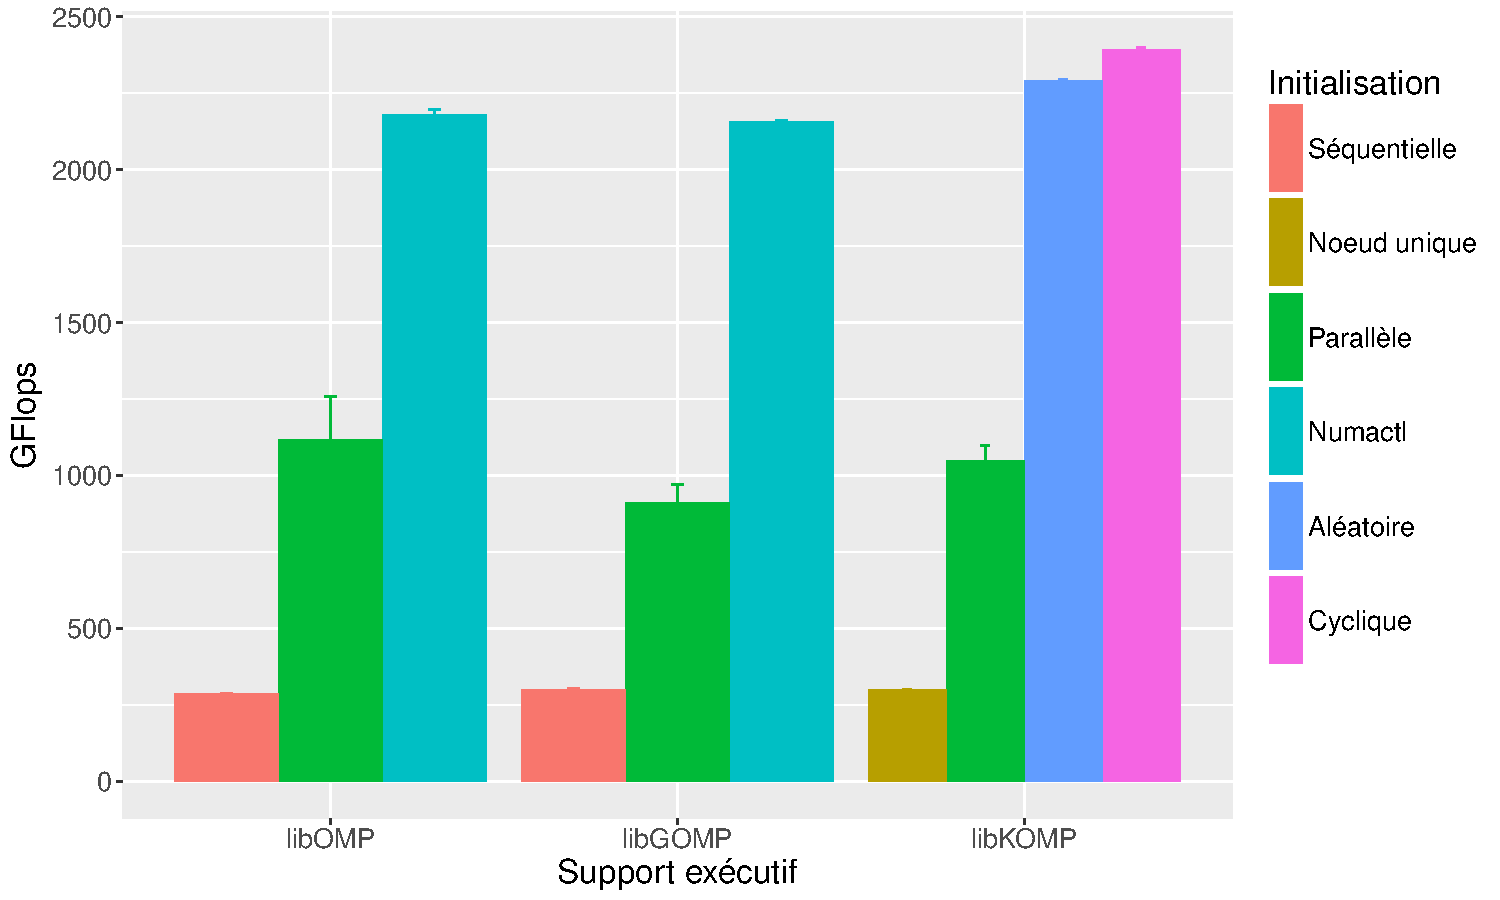
\includegraphics[width=\textwidth]{graph_distrib_data_idchire}
  \caption{Performances, sur les 192 cœurs d'idchire, des différentes stratégies pour Cholesky en fonction de la distribution de données. Taille de matrice~: 32768, taille de bloc~: 512}\label{fig:contribs:perf_eval:distrib-idchire}
\end{figure}


La figure~\ref{fig:contribs:perf_eval:distrib-idchire} montre un exemple représentatif du comportement de la factorisation de Cholesky par bloc, en fonction du support exécutif et du type de distribution de données. La taille de matrice utilisée est 32768, et la taille de bloc est 512, et la performance affichée est celle obtenue avec l'ensemble des 192 cœurs d'idchire.

La distribution \emph{Séquentielle} correspond à l'exécution du programme original.
La distribution \emph{Numactl} correspond à une distribution des pages des données effectuée de manière cyclique sur les nœuds de la machine à l'aide de \emph{numactl}.
Toutes les autres stratégies utilisent une initialisation parallèle dans laquelle chaque tâche est responsable de l'initialisation d'un bloc de données.

Parmi celles-ci, la distribution \emph{Non guidée} correspond à une distribution des tâches (et donc du placement des données, comme expliqué dans la section~\ref{sec:openmp:langage:init}) sur laquelle aucun contrôle n'a été effectué.
Néanmoins il y a une certaine distribution des tâches qui est naturellement effectuée~: compte tenu des tailles utilisées, il y a 64 blocs à initialiser et 24 nœuds sur la machine. En fonction de la rapidité d'initialisation du support exécutif et de l'ordre dans lesquels les threads commencent à travailler, cette distribution non guidée peut varier.

La distribution \emph{Nœud unique} correspond au placement de toutes les tâches d'initialisation sur un seul nœud (ce qui revient à faire une initialisation séquentielle).
Les deux autres distributions, \emph{Cyclique} et \emph{Aléatoire} correspondent aux distributions que nous avons implémentées, et distribuent les tâche de manière cyclique ou aléatoire sur les nœuds de la machine.

La première chose à remarquer est que l'initialisation séquentielle de base (ou l'initialisation sur un nœud unique) propose sans surprise des performances désastreuses.

L'initialisation parallèle \emph{Non guidée} se distingue par sa variabilité~: les barres d'erreurs illustrent cette variabilité, due à l'ordre dans lesquels les threads viennent voler les tâches d'initialisation.

Au final l'utilisation de \emph{numactl} permet de contrebalancer les effets de l'initialisation séquentielle et d'atteindre des performances raisonnables.

La différence entre \emph{Numactl} et une distribution \emph{Aléatoire} peut être expliquée par le fait que \emph{numactl} distribue les \emph{pages} de manière aléatoire, alors qu'une distribution aléatoire des tâches d'initialisation distribue des \emph{blocs de données}, composés de plusieurs pages.

Ajouter une distribution de données spécifique assure que la distribution des tâches ne repose pas sur l'ordonnancement par défaut du support exécutif, et l'ordre parfois non contrôlé dans lequel les threads viennent voler du travail.
Bien que la différence ne soit que de quelques dizaines de GFlops, la distribution \emph{Cyclique} sur l'ensemble des nœuds NUMA semble être plus avantageuse que la distribution \emph{Aléatoire} sur l'ensemble des stratégies d'ordonnancement testé, et c'est celle qu'on a retenu pour les expériences des sections suivantes.


\subsubsection{Étude de l'impact de l'affinité}

Dans cette section, les résultats de libKOMP ont été obtenus avec une distribution \emph{Cyclique} et avec une combinaison de stratégies prenant en compte l'affinité et les deux niveaux de hiérarchie des machines.
Nous avons étudié l'impact de l'affinité sous plusieurs angles~:

\paragraph{Performances brutes}

\begin{figure}[h!]
  \centering
  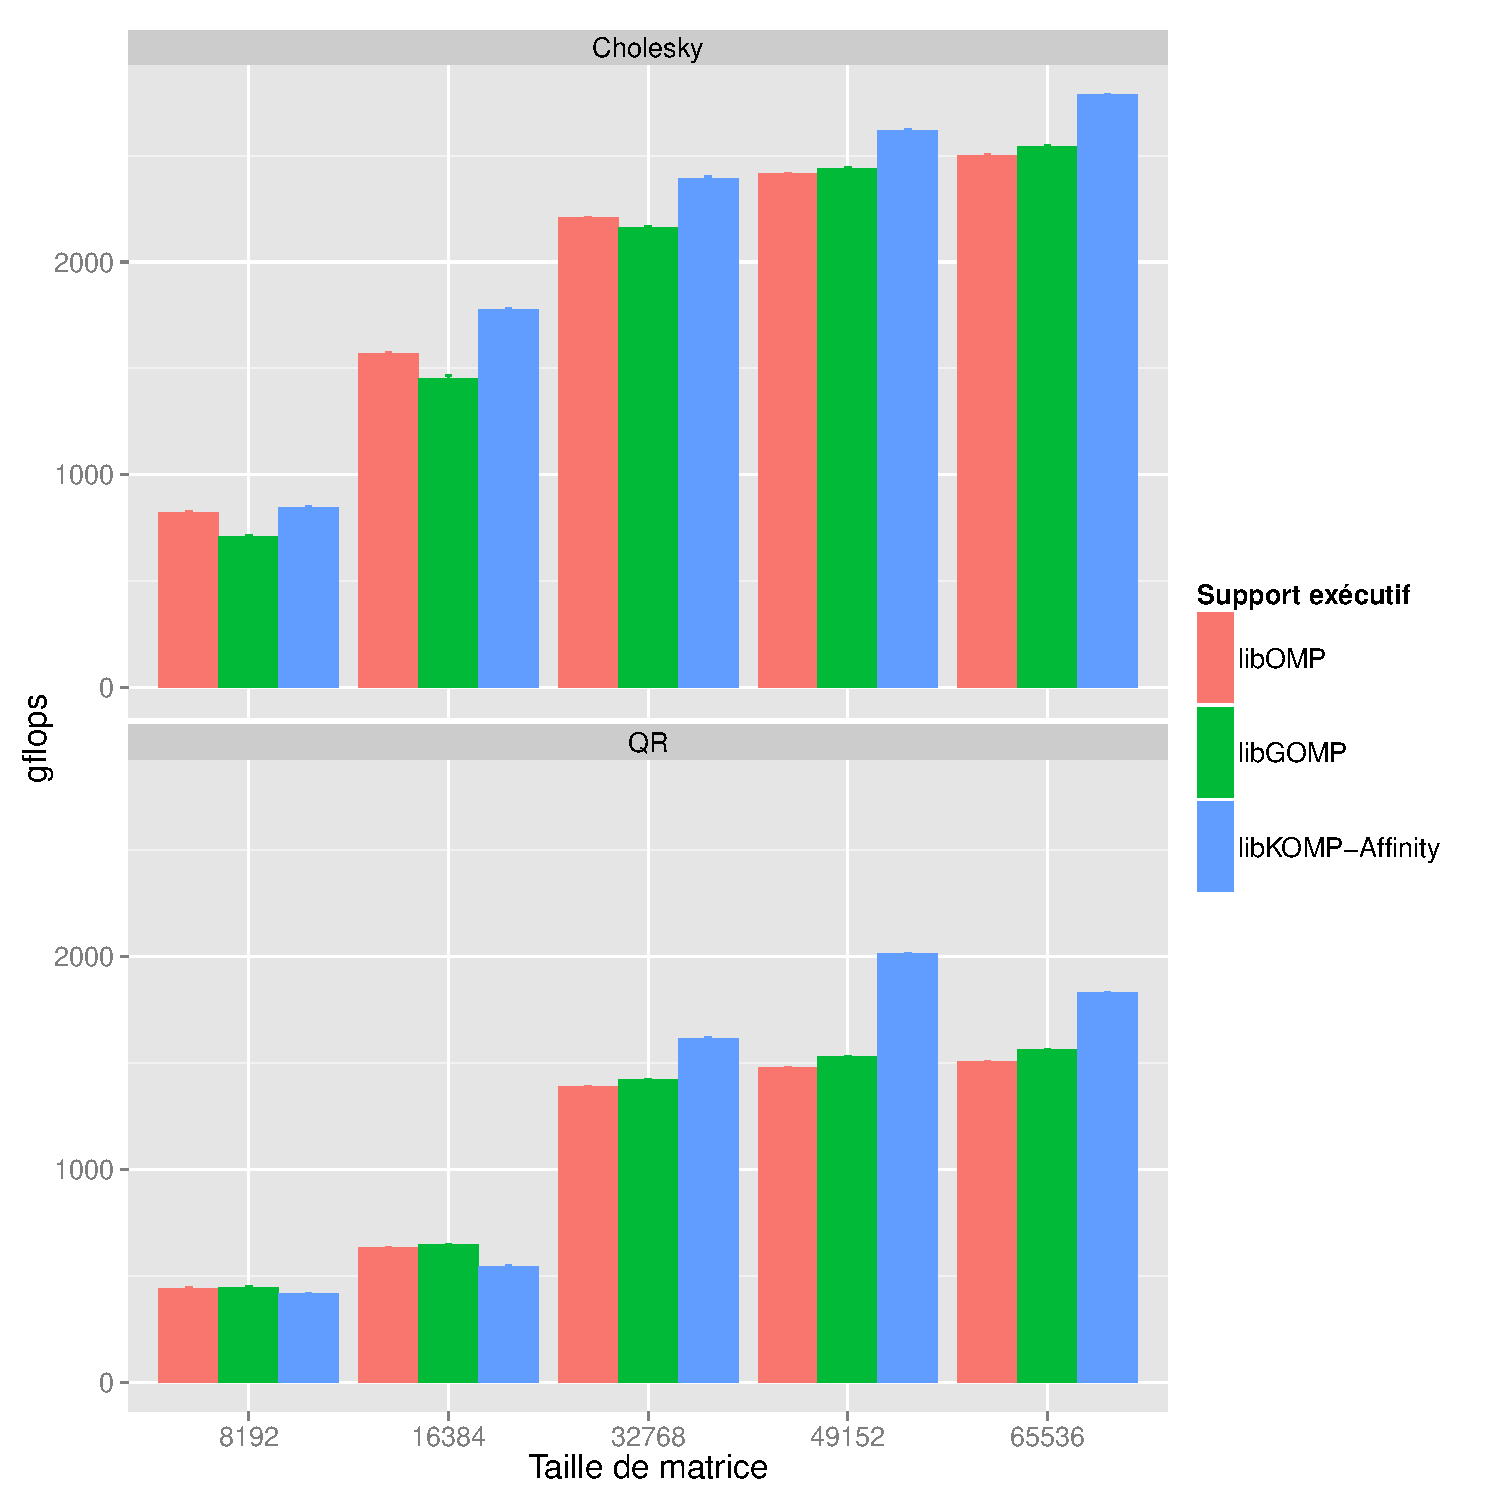
\includegraphics[width=\textwidth]{graph_details_qr_cholesky_idchire}
  \caption{Comparaison des supports exécutifs sur QR et Cholesky sur idchire, en fonction de la taille de matrice (tailles de bloc données dans le tableau~\ref{tab:perf_eval:blocksizes})}\label{fig:contribs:perf_eval:eval-qr-cholesky}
\end{figure}

Pour avoir un aperçu général des stratégies que nous avons évaluées sur les factorisations QR et Cholesky, avec des tailles de matrice variant entre 16384 et 65536~; les tailles de blocs correspondantes sont détaillées dans le tableau~\ref{tab:perf_eval:blocksizes}.

\begin{table}[h!]
\def\arraystretch{1.5}
\centering
\begin{tabular}{|c|c|c|c|c|c|}\hline
  Taille de matrice & 8192 & 16384 & 32768 & 49152 & 65536 \\\hline
  Taille de bloc & 256 & 256 & 512 & 512 & 512 \\\hline
\end{tabular}
\caption{Tableau de correspondance entre taille de matrice et taille de bloc}\label{tab:perf_eval:blocksizes}
\end{table}

\begin{figure}[h!]
  \centering
  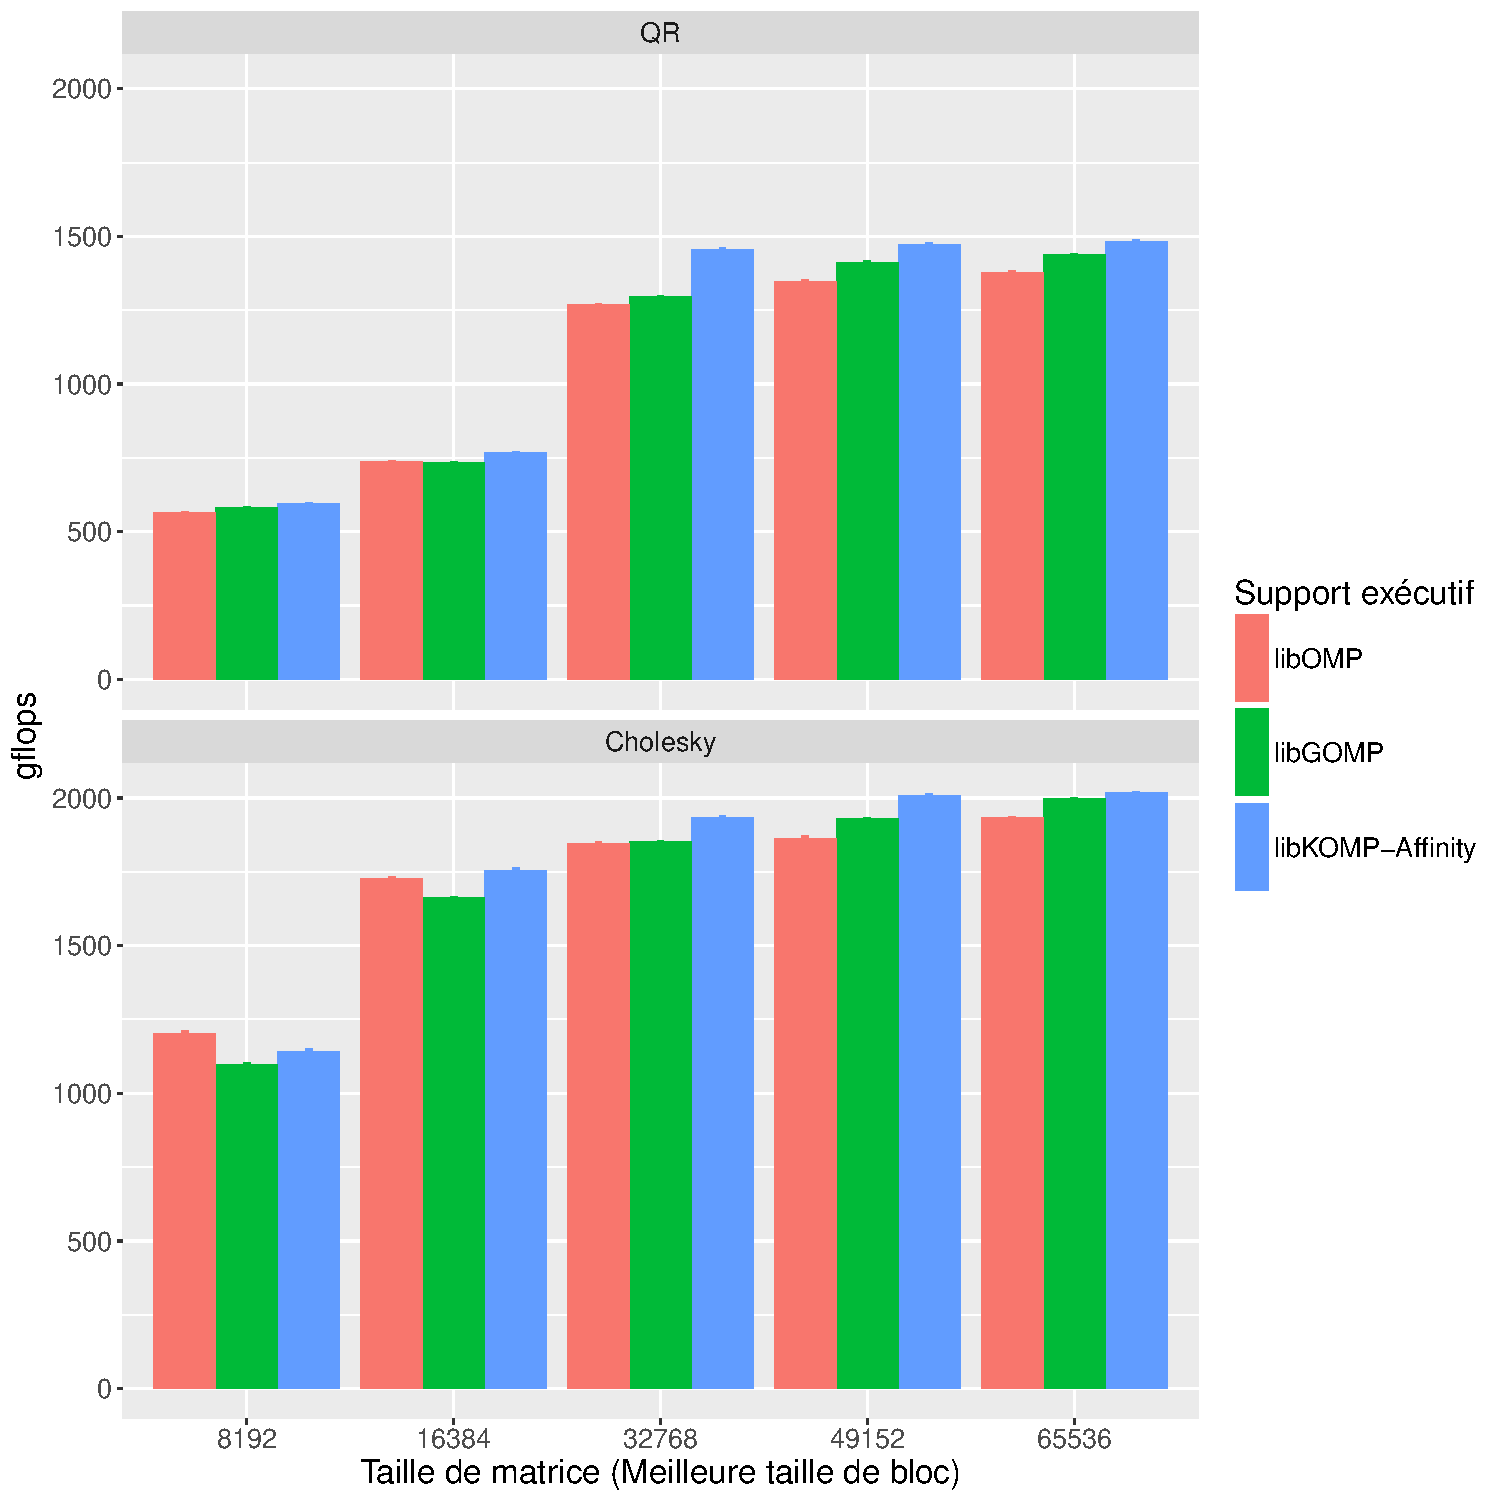
\includegraphics[width=\textwidth]{graph_details_qr_cholesky_brunch}
  \caption{Comparaison des supports exécutifs sur QR et Cholesky sur brunch, en fonction de la taille de matrice (tailles de bloc données dans le tableau~\ref{tab:perf_eval:blocksizes})}\label{fig:contribs:perf_eval:eval-qr-cholesky-brunch}
\end{figure}

La figure~\ref{fig:contribs:perf_eval:eval-qr-cholesky} montre les résultats obtenus sur idchire, et la figure~\ref{fig:contribs:perf_eval:eval-qr-cholesky-brunch} montre les résultats obtenus sur brunch.


Les machines brunch et idchire ont un facteur NUMA différent~: le coût d'accès à la mémoire distante par rapport à la mémoire locale est beaucoup plus important sur idchire que sur brunch.
Malgré cela, l'impact de l'affinité est bien visible sur les deux machines, même s'il est proportionnellement plus important sur idchire.

On peut observer que pour les faibles tailles de matrices, l'intérêt de l'affinité semble limité.
Plutôt que de regarder la taille de matrice, il faut en fait regarder la taille de bloc pour trouver l'explication de la différence~: pour les tailles de matrice 8192 et 16384 la taille de bloc est de 256, pour les autres elle de 512.
Les tailles de blocs induisent une différence claire vis à vis du cache L3~: dans le cas des blocs de taille 256 l'ensemble des données de calcul pour chaque noyau de l'application tient dans le cache L3, ce qui n'est pas le cas pour les blocs de taille 512.
Compte tenu des résultats montrés dans la section~\ref{sec:contribs:apps:cholesky:locality}, qui ont montré la dégradation très importante des performances lorsque les données ne tenant pas dans le cache sont à distance, il est donc logique d'observer l'amélioration significative des performances pour de grande tailles de blocs (nécessaires pour les grandes tailles de matrices), et une différence relativement faible concernant les tailles de blocs plus petites.


\paragraph{Évolution en fonction du nombre de cœurs}

La figure~\ref{fig:contribs:perf_eval:eval-cholesky-idchire} illustre l'évolution de l'impact de l'affinité en fonction du nombre de cœurs et de la taille de matrice sur idchire.


\begin{figure}[ht]
  \centering
  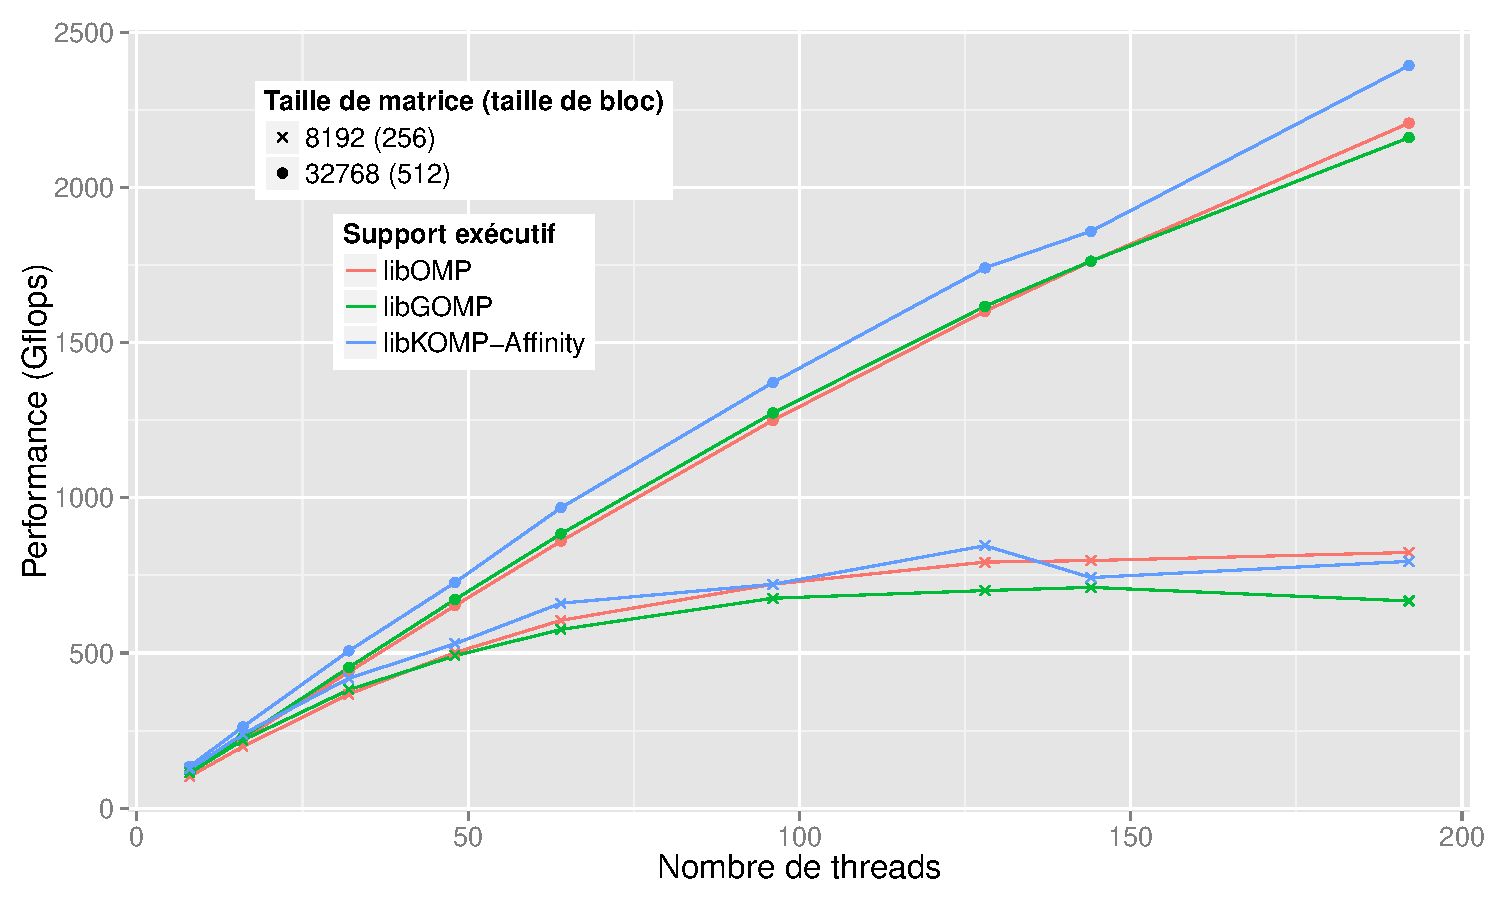
\includegraphics[width=\textwidth]{graph_all_cholesky_idchire}
  \caption{Performance en fonction du nombre de cœurs et de la taille de matrice sur idchire}\label{fig:contribs:perf_eval:eval-cholesky-idchire}
\end{figure}

Comme pour les expériences précédentes, les tailles de blocs correspondantes sont 256 pour la taille 8192, et 512 pour la taille 32768.
Les deux tailles de matrice choisies représentent les deux situations décrites précédemment~: dans un cas les données des noyaux de Cholesky tiennent dans le cache L3, dans l'autre non.
Dans le cas d'une petite taille de bloc on peut constater que la courbe de libKOMP se situe entre libOMP et libGOMP, ne donnant donc aucun résultat concluant, voire même étant coûteux par rapport à un simple vol de travail aléatoire comme dans libOMP !
Pour une grosse taille de bloc en revanche c'est clair et net~: après avoir suivi le même départ, les courbes divergent. Les supports exécutif libOMP et libGOMP affichent les même performances, tandis que l'affinité offre un net gain.

\begin{figure}[t!]
  \centering
  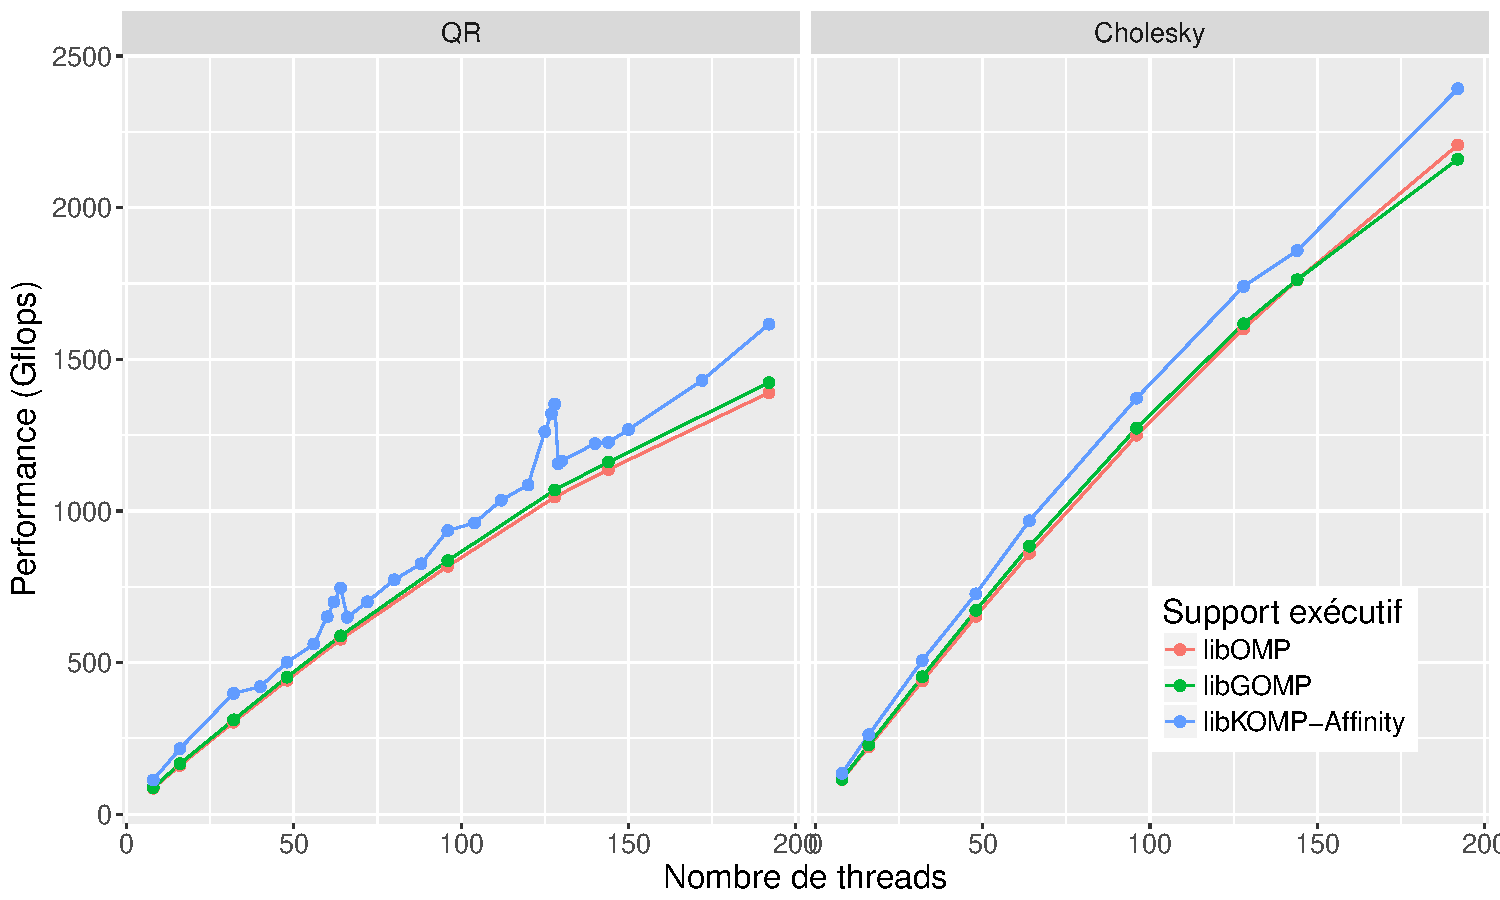
\includegraphics[width=\textwidth]{graph_qr_cholesky_vs_threads}
  \caption{Performance de QR et Cholesky en fonction du nombre de cœurs sur idchire. Taille de matrice~: 32768, taille de bloc~: 512}\label{fig:contribs:perf_eval:eval-qr-cholesky-idchire}
\end{figure}
\begin{figure}[h!]
  \centering
  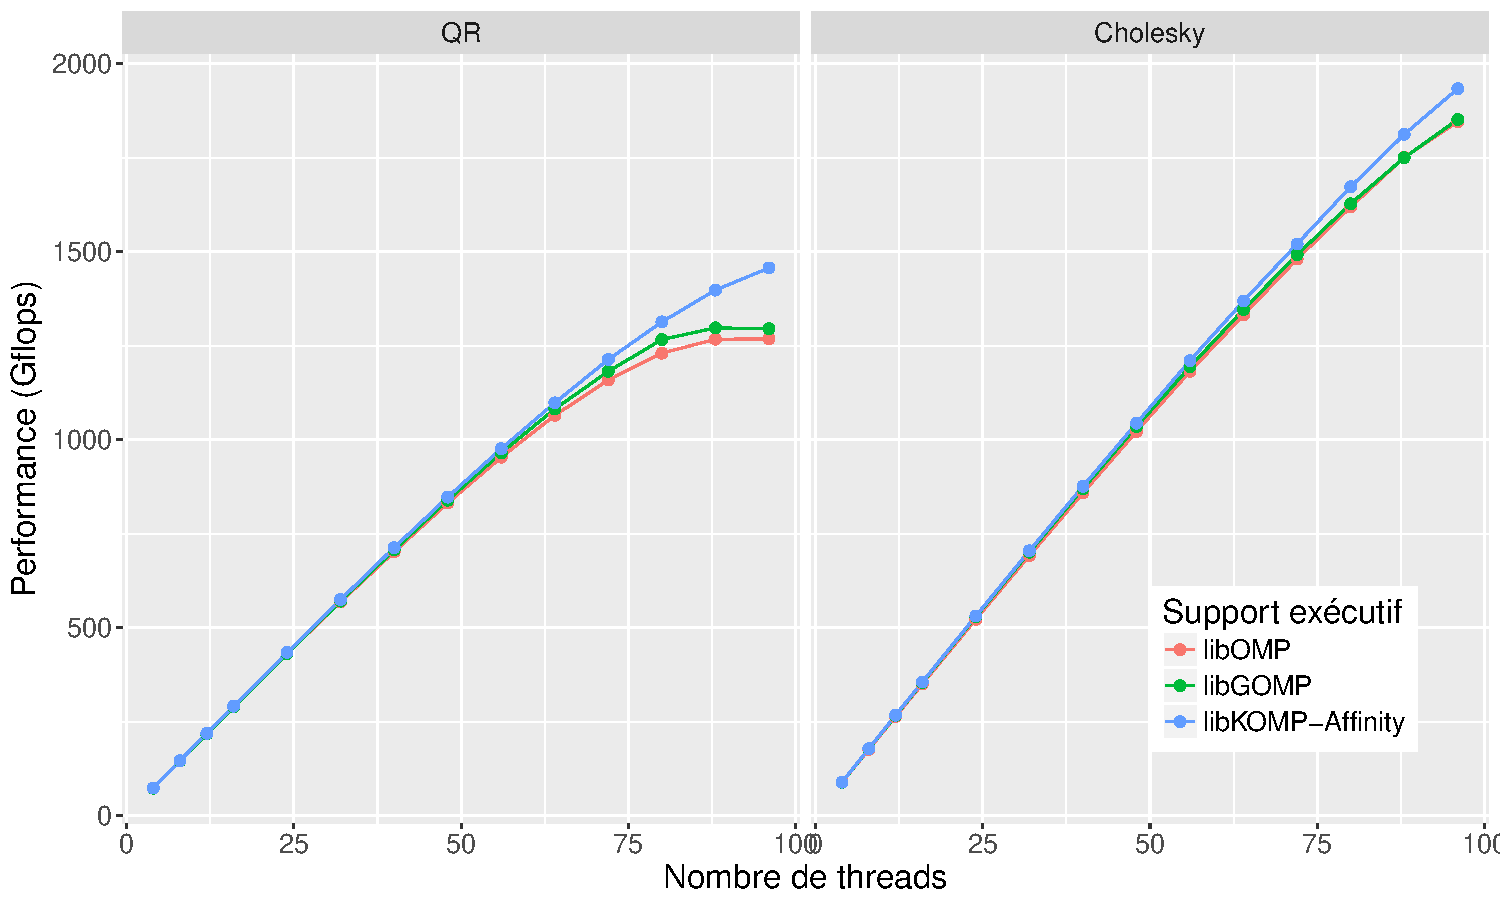
\includegraphics[width=\textwidth]{graph_qr_cholesky_vs_threads_brunch}
  \caption{Performance de QR et Cholesky en fonction du nombre de cœurs sur brunch. Taille de matrice~: 32768, taille de bloc~: 512}\label{fig:contribs:perf_eval:eval-qr-cholesky-brunch}
\end{figure}

Les figures~\ref{fig:contribs:perf_eval:eval-qr-cholesky-idchire} et~\ref{fig:contribs:perf_eval:eval-qr-cholesky-brunch} montrent les résultats des factorisations QR et Cholesky (taille de matrice 32768, taille de bloc 512) en fonction du nombre de threads sur idchire et brunch, respectivement.
Comparer les mêmes instances sur les deux machines donne des résultats intéressants~: leurs caractéristiques ne changent pas l'allure général des courbes, en revanche le faible facteur NUMA de brunch fait bien sentir que l'affinité n'est rentable que lorsque la machine est chargée à partir d'un seuil élevé (environ 75\%).
Alors que sur idchire la différence se voit dès une trentaine de cœur (qui correspond d'ailleurs à 4 nœuds NUMA).

En faisant ces expériences nous avons constaté un comportement assez atypique de QR avec l'affinité~: il y a 3 petits pics de performances à 32, 64, et 128 cœurs (soit 4, 8, et 16 nœud NUMA) !
Nous n'avons pas pu faire une étude aussi approfondie de QR que de Cholesky, il est donc dur d'expliquer ce comportement qui doit être dû à certaines caractéristiques de l'application.

%mais ici on peut penser que la distribution des données est responsable de ces pics. La distribution utilisée est cyclique, et sur un nombre de nœud NUMA en puissance de 2 cela doit fournir des propriétés favorables à l'application.



\subsubsection{Affinité stricte}

La section~\ref{sec:openmp:langage:affinity} introduit la clause affinité en précisant que l'utilisateur peut spécifier une affinité \emph{stricte}, restreignant ainsi les décisions d'ordonnancement du support exécutif.
Cette fonctionnalité n'a pas été utilisée pour les applications d'algèbre linéaire, car dans les cas que nous avons étudiés il était plus rentable de payer le coût de transfert des blocs de données plutôt que de se priver du parallélisme disponible.
Ce n'est évidemment pas le cas pour toutes les applications, et les applications stencil, comme Jacobi, peuvent grandement bénéficier d'une restriction d'affinité aux ressources proches, du fait de leur faible intensité opérationnelle (dans le cas de Jacobi, elle est en $O(1)$).

\begin{figure}[ht]
  \centering
  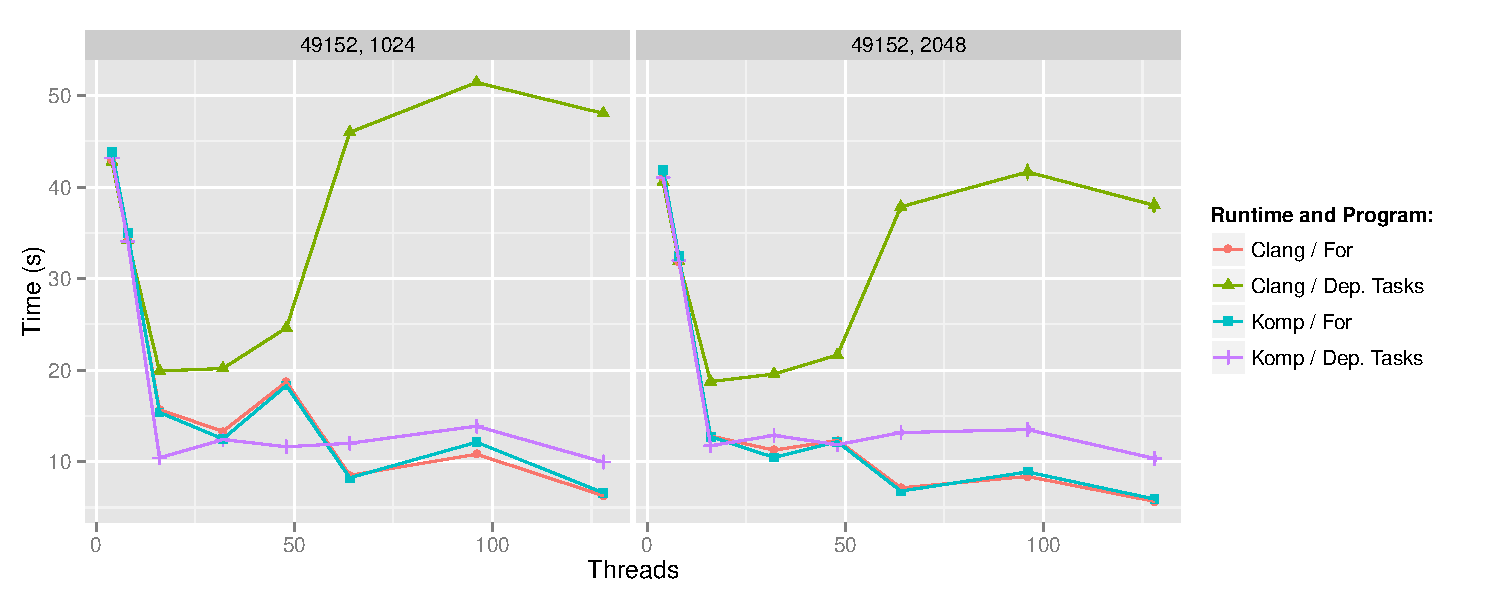
\includegraphics[width=\textwidth]{jacobi_scale_iomp_komp}
  \caption{Performances de Jacobi en fonction de la version et du support exécutif, avec une taille de matrice de 49152, sur idchire}\label{fig:contribs:perf_eval:eval-jacobi}
\end{figure}

La figure~\ref{fig:contribs:perf_eval:eval-jacobi} montre les performances de Jacobi sur deux tailles de blocs différentes.
Les mesures avec l'affinité ont été effectuées avant le portage dans libOMP, et le support exécutif sous-jacent est donc XKaapi.
La version à base d'OpenMP |for| utilise un ordonnancement statique, sans contrôle particulier sur la distribution des données.
Les versions à base de tâches avec dépendances n'utilisent aucun contrôle sur le placement des tâches ou des données.
Pour la version avec affinité, une distribution de données a été rajoutée dans l'application, avec également une affinité stricte suivant cette distribution de données sur les itérations successives.
Cette distribution affecte les blocs de données sur une grille la plus carrée possible en fonction des nœuds utilisés.
L'affinité stricte ajoutée permet de garantir la réutilisation des données présentes dans le cache L2 (point critique pour cette application), et éviter des migrations de tâches inappropriées, ce qui est d'autant plus important que l'intensité opérationnelle est faible.
Les performances obtenues avec les versions à base de boucles sont faibles comparativement aux résultats de l'affinité, néanmoins cela vient du fait qu'il n'y a pas eu d'effort particulier de fait pour que le découpage des itérations correspondent à celui des distributions des données.
Les performances des deux versions devraient théoriquement être équivalentes~: l'affinité stricte est là pour restreindre la portée du vol de travail qui dégradait les performances, phénomène qui ne devrait pas être présent dans une version à base de boucles.
\begin{todo}
  est-ce que je parle de la version for+affinité, qui matche la version tâche+affinité ?
\end{todo}


\section{Dicussions et conclusion}
\subsection{Implémenter ces idées dans d'autres supports exécutifs}

\subsection{Quelles sont les prochaines étapes ?}
More flexibility for initialization


